\section{Adressprotokolle}

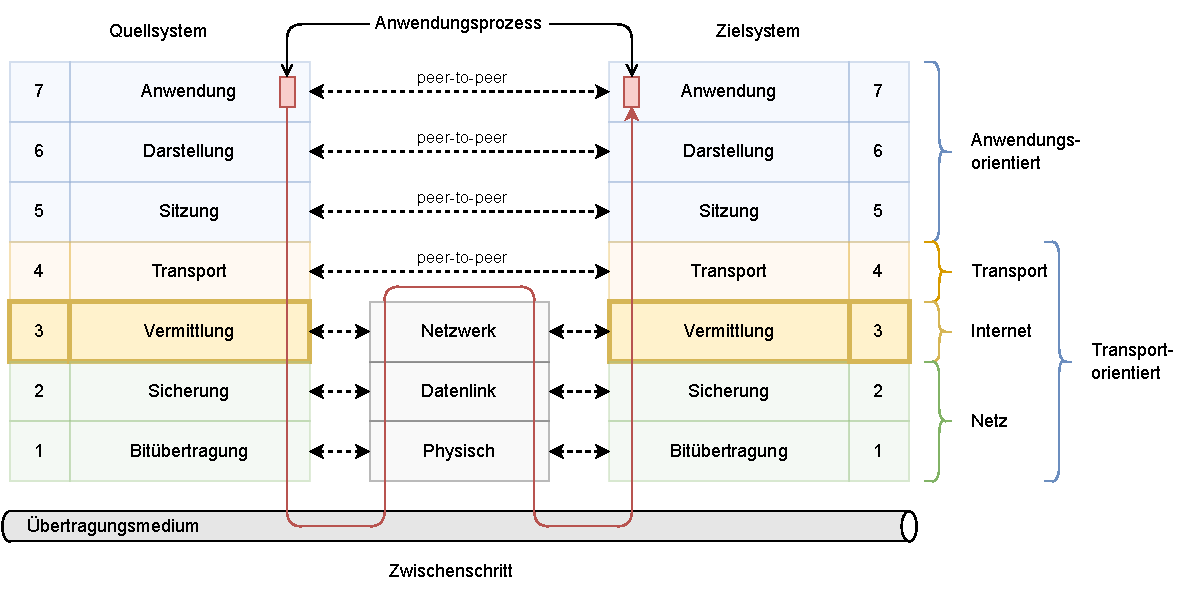
\includegraphics[width=\textwidth]{includes/figures/defi_iso_osi_vermittlung.pdf}

\subsection{ARP, RARP}

\begin{defi}{MAC-Adresse}
    \begin{center}
        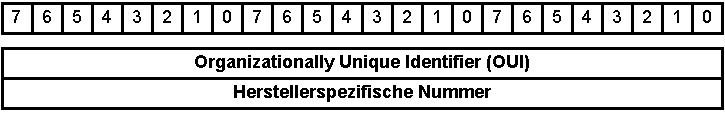
\includegraphics[width=0.5\textwidth]{includes/figures/defi_mac.pdf}
    \end{center}

    Die \emph{MAC-Adresse} ist die Hardware-Adresse jedes einzelnen Netzadapters, die als eindeutiger Identifikator des Geräts in einem Rechnernetz dient.
    Man spricht auch von physischer Adresse oder Geräteadresse.\footnote{Bei Apple wird sie Ethernet-ID, Airport-ID oder Wi-Fi-Adresse genannt, bei Microsoft Physikalische Adresse.}

    Die MAC-Adresse enthält neben einer ID lediglich Informationen zum Hersteller, weshalb kein Routing mithilfe der MAC-Adresse möglich ist.

    Die Broadcast-Adresse ist definiert als \texttt{FF:FF:FF:FF:FF:FF} definiert.

\end{defi}

\begin{defi}{ARP}
    Das \emph{Address Resolution Protocol (ARP)} ist ein Netzwerkprotokoll, das zu einer Netzwerkadresse der Internetschicht die physische Adresse (MAC-Adresse) der Netzzugangsschicht ermittelt und diese Zuordnung gegebenenfalls in den \emph{ARP-Tabellen} der beteiligten Rechner hinterlegt.

    Der Ablauf ist z. B. bei Ethernet wie folgt:\footnote{Für ARP-Request und ARP-Reply wird das gleiche Paketformat verwendet.}
    \begin{enumerate}
        \item Es wird eine \emph{ARP-Request} mit MAC-Adresse und IP-Adresse des anfragenden Rechners als Quelle und der IP-Adresse des gesuchten Empfängers als Ziel an alle Computer des lokalen Netzwerkes gesendet.
        \item Empfängt ein Computer ein solches Paket, sieht er nach, ob dieses Paket seine IP-Adresse als Empfänger-IP-Adresse enthält.\footnote{Zusätzlich können die Empfänger des ARP-Requests ebenfalls die Kombination von IP-Adresse und MAC-Adresse des anfragenden Computers in ihre ARP-Tabelle eintragen bzw. einen bestehenden Eintrag aktualisieren. Insbesondere der Rechner mit der im ARP-Request angefragten IP-Adresse sollte diese Eintragung vornehmen, da anzunehmen ist, dass der ARP-Request als Vorbereitung für weitere Kommunikation auf höherer Protokollebene dienen soll, wofür er dann für eventuelle Antworten ebenfalls die MAC-Adresse des Anfragenden benötigt.}
        \item Wenn dies der Fall ist, antwortet er mit dem Zurücksenden seiner MAC-Adresse und IP-Adresse (\emph{ARP-Reply}) per Broadcast oder als Unicast.
        \item Der Empfänger trägt nach Empfang der Antwort die empfangene Kombination von IP- und MAC-Adresse in seine ARP-Tabelle, auch ARP-Cache genannt, ein.
    \end{enumerate}
\end{defi}

\begin{bonus}{ARP-Paket}
    \centering
    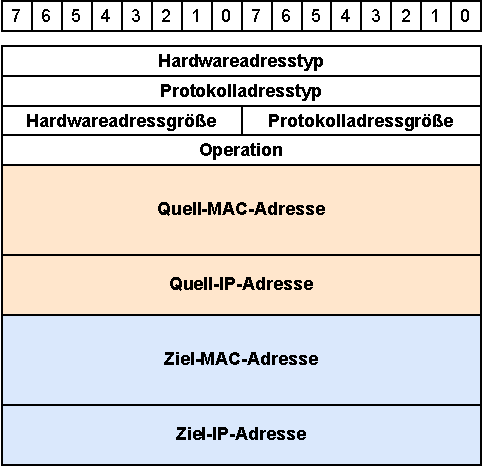
\includegraphics[width=.5\textwidth]{includes/figures/defi_arp_paket.pdf}
\end{bonus}

\begin{example}{ARP}
    Der Computer mit MAC-Adresse \texttt{7B:87:32:1E:74:72} und IP-Adresse \texttt{192.168.0.22} sucht die MAC-Adresse zum Computer mit der IP-Adresse \texttt{192.168.0.5}.\footnote{Die ARP-Reply wird dann auch über die gestrichelten Routen versandt, wenn Broadcast verwendet wird. Wird Unicast verwendet, gelangt die ARP-Reply nur an den ursprünglichen Sender.}

    \centering
    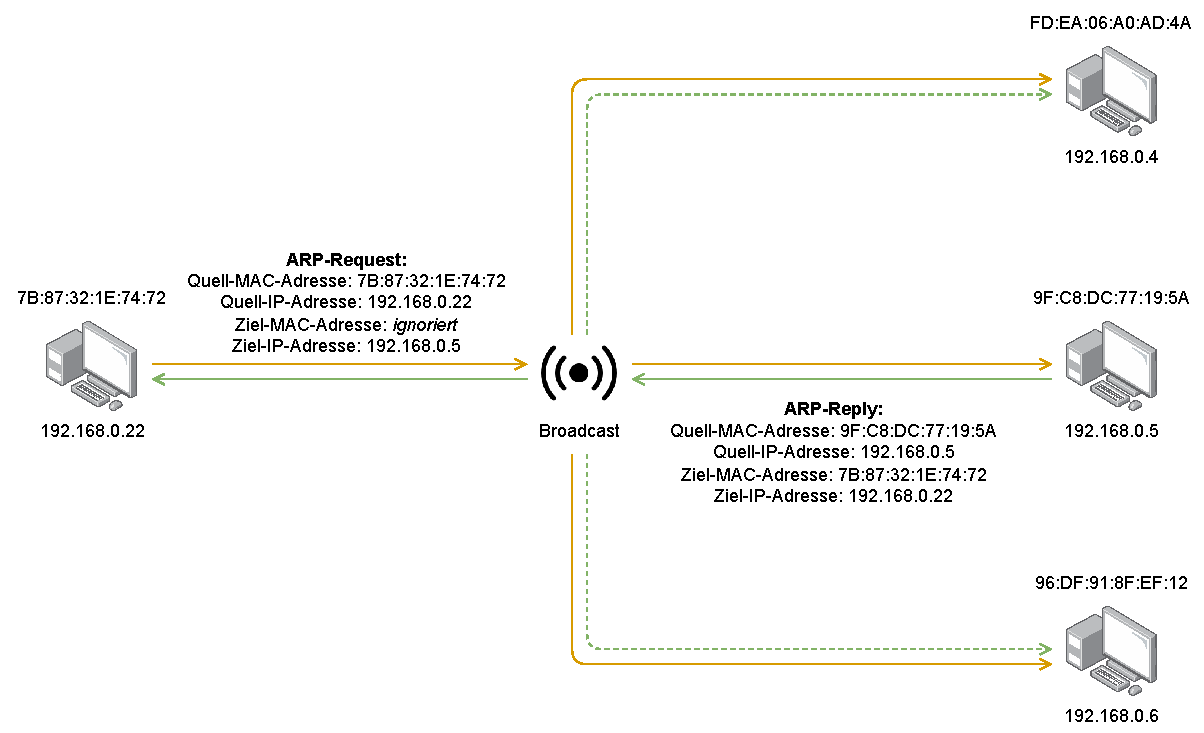
\includegraphics[width=\textwidth]{includes/figures/example_arp.pdf}
\end{example}

\begin{defi}{RARP}
    Das \emph{Reverse Address Resolution Protocol (RARP)} ist ein Netzwerkprotokoll, das die Zuordnung von Hardwareadressen zu Internetadressen ermöglicht.

    RARP sendet dazu ein \emph{RARP-Request}-Broadcast mit der eigenen MAC-Adresse als Inhalt an die am Netzwerk angeschlossenen Rechner.
    Ein RARP-Server, welcher alle Zuordnungen IP- zu MAC-Adressen kennt, sendet daraufhin eine Antwort mit der IP-Adresse an die anfragende MAC-Adresse (\emph{RARP-Reply}).
\end{defi}

\begin{bonus}{Probleme von RARP}
    Die vermeintliche Eindeutigkeit der MAC-Adresse darf nicht als Sicherheitskriterium angewandt werden. Es ist viel zu einfach, MAC-Adressen-Spoofing zu betreiben.

    Gültige MAC-Adressen in einem Schicht-2-Netz können durch Abhören des Netzverkehrs ausfindig gemacht werden. Dazu ist lediglich der physische Zugang zum Netzwerk nötig.
    Die exklusive Vergabe von IP-Adressen nur an registrierte MAC-Adressen über RARP oder DHCP schließt also nicht aus, dass Unberechtigte Zugriff auf das Netzwerk erhalten.

    Außerdem sind Ethernet-Broadcasts auf Subnetze beschränkt, so dass RARP nur in einem Subnetz eingesetzt werden kann.
    Wird ein lokales Netzwerk (LAN) in Subnetze aufgeteilt, muss in jedem dieser Subnetze, in dem RARP-fähige Terminals oder Workstations eingesetzt werden, ein eigener RARP-Server vorhanden sein.
\end{bonus}

\subsection{DHCP}

\begin{defi}{DHCP}
    Das \emph{Dynamic Host Configuration Protocol (DHCP)} ermöglicht es, angeschlossene Clients ohne manuelle Konfiguration der Netzschnittstelle in ein bestehendes Netz einzubinden.

    Nötige Informationen wie IP-Adresse, Netzmaske, Gateway, Name Server (DNS) und ggf. weitere Einstellungen werden automatisch vergeben, sofern das Betriebssystem des jeweiligen Clients dies unterstützt.
\end{defi}

\begin{defi}{DHCP-Betriebsmodi}
    Es gibt drei verschiedene Betriebsmodi eines DHCP-Servers:
    \begin{itemize}
        \item \emph{Statische Zuordnung} bzw. \emph{statisches DHCP}:
              \begin{itemize}
                  \item Am DHCP-Server werden IPs bestimmten MAC-Adressen fest zugeordnet.
                  \item Adressen werden der MAC-Adresse auf unbestimmte Zeit zugeteilt.
                  \item Nachteil kann darin liegen, dass sich keine zusätzlichen Clients in das Netz einbinden können.\footnote{Das kann unter Sicherheitsaspekten erwünscht sein.}
              \end{itemize}
        \item \emph{Automatische Zuordnung}:
              \begin{itemize}
                  \item Am DHCP-Server wird ein Bereich von IP-Adressen (range) definiert.
                  \item IP-Adressen werden automatisch an die MAC-Adressen von neuen DHCP-Clients zugewiesen, was in einer Tabelle festgehalten wird.
                  \item Im Unterschied zur dynamischen Zuordnung sind automatische Zuordnungen permanent und werden nicht entfernt.
                  \item Vorteil ist, dass Hosts immer dieselbe IP-Adresse erhalten und eine zugewiesene IP-Adresse keinem anderen Host zugewiesen wird.
                  \item Nachteil ist, dass neue Clients keine IP-Adresse erhalten, wenn der gesamte Adressbereich vergeben ist, auch wenn IP-Adressen nicht mehr aktiv genutzt werden.
              \end{itemize}
        \item \emph{Dynamische Zuordnung}:
              \begin{itemize}
                  \item Gleicht der automatischen Zuordnung, allerdings hat der DHCP-Server hier in seiner Konfigurationsdatei eine Angabe, wie lange eine bestimmte IP-Adresse an einen Client verliehen werden darf, bevor der Client sich erneut beim Server melden und eine Verlängerung beantragen muss.
                  \item Meldet er sich nicht, wird die Adresse frei und kann an einen anderen (oder auch denselben) Rechner neu vergeben werden. Diese vom Administrator bestimmte Zeit heißt \emph{Lease-Time}.
              \end{itemize}
    \end{itemize}
\end{defi}

\begin{bonus}{DHCP-Paket}
    \centering
    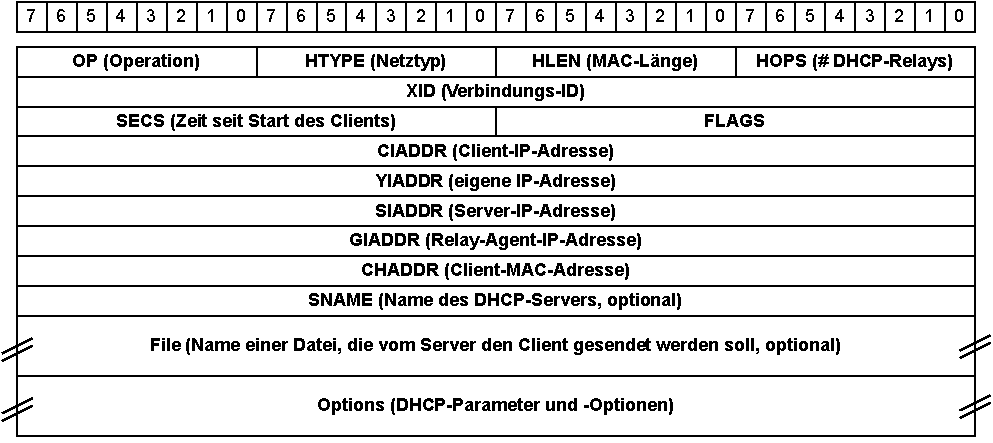
\includegraphics[width=.75\textwidth]{includes/figures/defi_dhcp_paket.pdf}
\end{bonus}

\subsection{Fragmentierung}

\begin{defi}{IPv4-Header}
    \centering
    
\includegraphics[width=0.75\textwidth]{includes/figures/defi_ip_header_kapselung.pdf}

    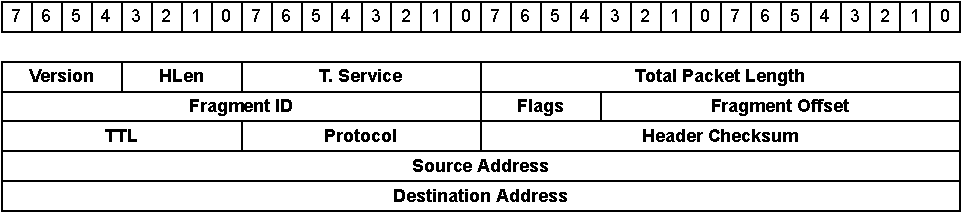
\includegraphics[width=0.75\textwidth]{includes/figures/defi_ip_header.pdf}
\end{defi}

\begin{defi}{IP-Fragmentierung}
    Die \emph{IP-Fragmentierung} bezeichnet die Aufteilung eines IP-Datenpakets auf mehrere Datenblöcke, falls die Gesamtlänge des Datenpakets größer als die \emph{Maximum Transmission Unit (MTU)} der Netzwerkschnittstelle ist.

    Wird ein IP-Datagramm fragmentiert, so wird es erst beim Empfänger wieder zusammengesetzt.\footnote{Ausnahme: ggf. zwischengeschaltete Firewalls, die speziell angewiesen wurden, ein sogenanntes reassembly durchzuführen, bevor die Daten weitergeleitet werden.}
    Sollte es nötig sein, kann auch ein bereits fragmentiertes Paket weiter fragmentiert werden (etwa bei einem Wechsel der Übertragungstechnik).

    Jedes IP-Datagramm, das fragmentiert wurde, erhält einen neuen Header auf Basis des originalen Headers und spezieller aktualisierter Felder.

    In den neuen IP-Headern der Fragmente gibt der \emph{Offset} die Position der in diesem Paket versendeten Daten in Relation zum Originalpaket an (wird in 8-Byte-Blöcken angegeben).

    Wichtig: Dadurch müssen alle Fragmente (bis auf das letzte) eine durch 8 teilbare Größe haben.
\end{defi}

\begin{example}{IP-Fragmentierung}
    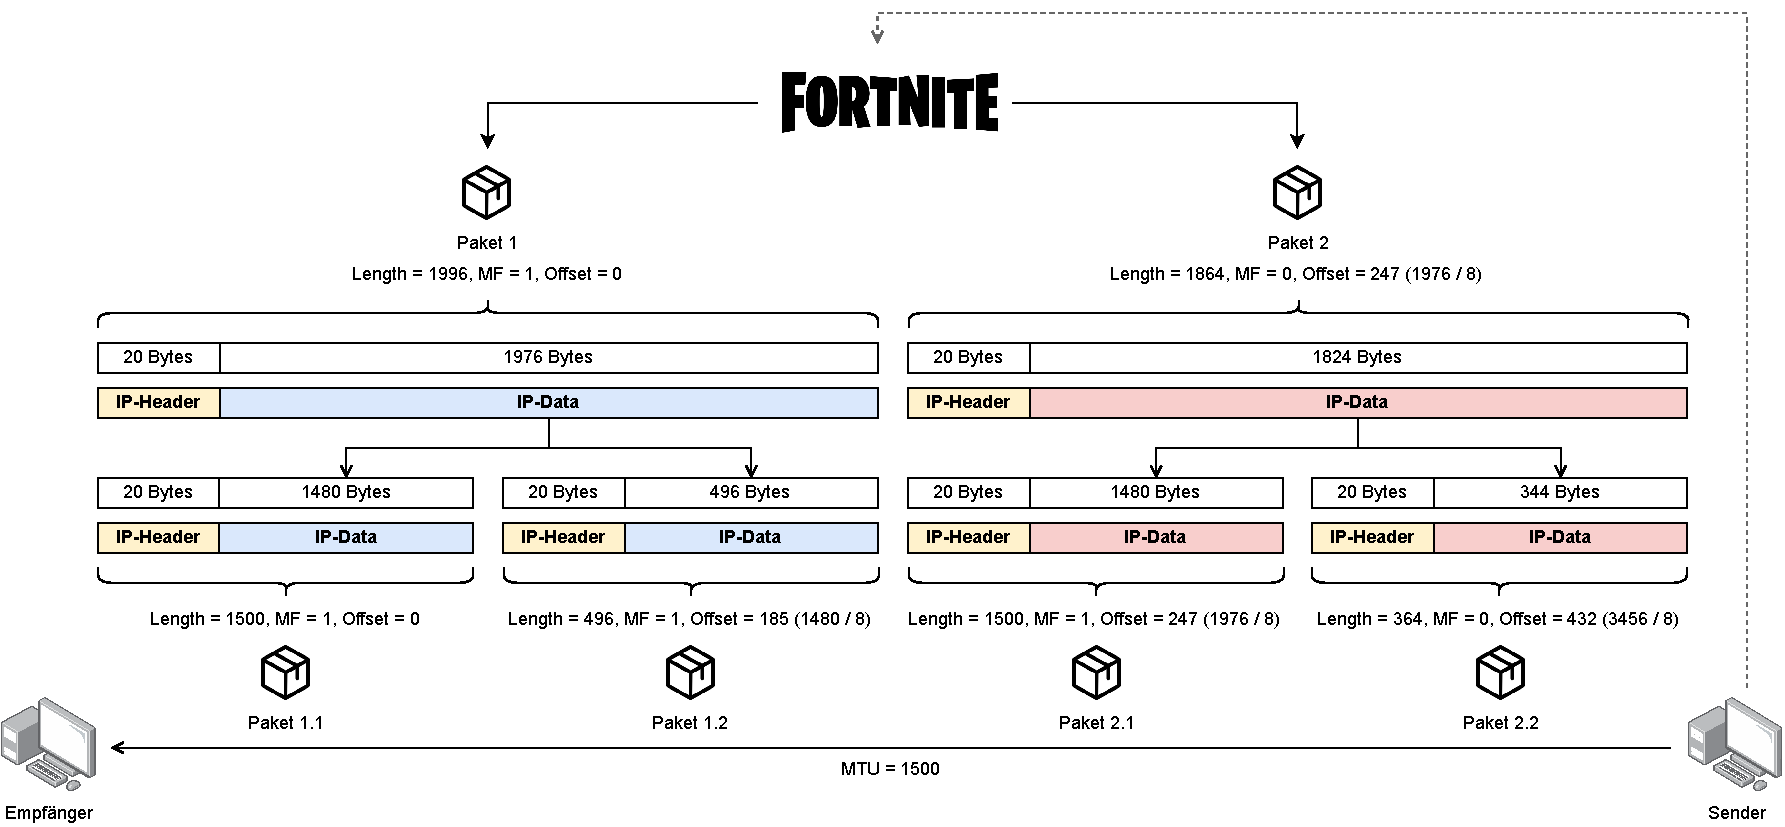
\includegraphics[width=\textwidth]{includes/figures/example_fragmentierung.pdf}
\end{example}

\begin{bonus}{Zusammensetzen der Fragmente}
    Der Empfänger hat nun die Aufgabe, das Original aus den in den Paketheadern vorhandenen Informationen wieder zusammenzusetzen, indem er alle Fragmente mit gleichem IP-Header (mit Ausnahme der für jedes Fragment separaten Information) nimmt und sie anhand ihres Offsets in die richtige Reihenfolge bringt.

    Da jedes einzelne Fragment ein eigenständiges Paket darstellt, kann es auch vorkommen, dass diese Einzelteile nicht geordnet ankommen.

    Es ist auch möglich, dass einzelne Fragmente verlorengehen oder defekt sind.
    Es ist dann Sache des Empfängers, das Paket zu verwerfen und die Daten erneut anzufordern, wodurch eine höhere Netzwerklast entstehen kann.
\end{bonus}

\begin{defi}{Path MTU Discovery}
    \emph{Path MTU Discovery} ist ein Verfahren zum dynamischen Erkennen der Maximum Transmission Unit (MTU) und damit der maximalen Paketgröße für einen bestimmten Pfad im Netzwerk.

    Im Allgemeinen kann mit dieser Information Overhead vermindert und Fragmentierung von Datenpaketen verhindert werden.

    Um in IPv4-Netzen die maximale Größe zu bestimmen, die ein Datenpaket haben sollte, muss die Stelle des Pfades gefunden werden, die die kleinsten Datenpakete zulässt.

    Vorgehen\footnote{Nur gültig in IPv4, da in IPv6 keine Fragmentierung von weitergeleiteten Paketen auf Routern stattfindet.}:
    \begin{enumerate}
        \item Es wird ein IPv4-Paket versendet, bei dem das \texttt{DF}-Bit (Don't Fragment) gesetzt ist und das die Größe der lokal eingestellten Maximum Transmission Unit hat.
        \item Kommt das Paket an eine Stelle im Netz, an dem nur eine kleinere MTU verarbeitet werden kann, wird ein ICMP-Error Typ 3 Code 4 (Destination Unreachable Fragmentation Needed, DF Set) zurückgeschickt, der auch die eigene MTU enthält.
        \item Der lokale Rechner erhält dieses ICMP-Paket und kann die Größe seiner Nachrichten nun an die zurückgeschickte MTU anpassen.
        \item Wiederhole, bis das Paket den gesamten Pfad ohne Fragmentierung durchlaufen kann.
    \end{enumerate}
\end{defi}

\begin{bonus}{Jumbo Frames}
    Der Begriff \emph{Jumbo Frames} bezeichnet nicht standardisierte Frames (d. h. Zusammenfassungen der zu übertragenden Daten), die größer sind als die in der Norm IEEE 802.3 festgelegte Standardgröße von 1518 Bytes.

    Für einige Anwendungen können Jumbo Frames sinnvoll sein, da durch sie der Protokoll-Overhead reduziert und die Effizienz verbessert werden können.

    Außerdem kann bei den beteiligten Knoten der Verarbeitungsoverhead möglicherweise gesenkt werden, da weniger Frames verarbeitet werden müssen.

    Solche Frames sind nicht Standard, und so muss sichergestellt werden, dass alle Netzwerkelemente wie Switches, Router etc. in einem Netz mit diesen Jumbo Frames umgehen können, und getestet werden, ob es einen Geschwindigkeitsvorteil gibt.
\end{bonus}

\subsection{ICMP}

\begin{defi}{ICMP}
    Das \emph{Internet Control Message Protocol (ICMP)} dient dem Austausch von Informations- und Fehlermeldungen über das Internet-Protokoll in der Version 4 (IPv4). Für IPv6 existiert ein ähnliches Protokoll mit dem Namen ICMPv6.

    ICMP ist Bestandteil von IPv4, wird aber wie ein eigenständiges Protokoll behandelt.
    Es wird von jedem Router und jedem Rechner erwartet, dass sie ICMP verstehen.

    Die meisten ICMP-Pakete enthalten Diagnose-Informationen: Sie werden vom Router zur Quelle zurückgeschickt, wenn der Router Pakete verwirft, etwa weil beispielsweise das Ziel nicht erreichbar ist oder die TTL abgelaufen ist.

    Es gelten folgende Grundsätze:
    \begin{itemize}
        \item ICMP benutzt IP als Kommunikationsbasis, indem es sich selbst als Protokoll einer höheren Schicht interpretiert, d. h. ICMP-Nachrichten werden in IP-Paketen gekapselt.
        \item ICMP erkennt einige Fehlerzustände, macht aber IP zu keinem zuverlässigen Protokoll.
        \item ICMP analysiert Fehler in jedem IP-Paket, mit Ausnahme solcher, die eine ICMP-Nachricht tragen.
        \item ICMP-Nachrichten werden nicht als Antwort auf Pakete an Zieladressen versendet, bei denen es sich um Multicast- oder Broadcast-Adressen handelt.
        \item ICMP-Nachrichten antworten nur einer eindeutigen Quell-IP-Adresse.
    \end{itemize}

    Beispiele für Nachrichtentypen:
    \begin{itemize}
        \item \emph{Destination Unrechable}: Ziel nicht erreichbar
        \item \emph{Time Exceeded}: Time-to-Live-Feld eines Pakets ist abgelaufen
        \item \emph{Echo Reply}: Echo-Reply wird angefordert (\texttt{ping})
    \end{itemize}
\end{defi}

\begin{defi}{ICMP-Header}
    \centering
    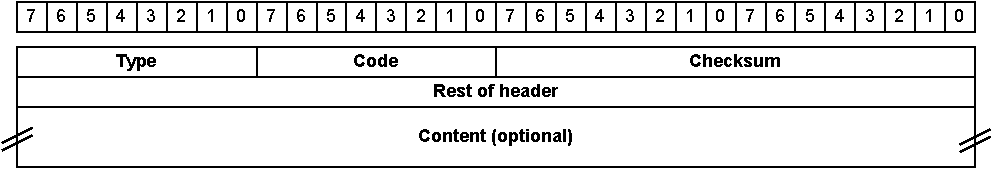
\includegraphics[width=.75\textwidth]{includes/figures/defi_icmp_header.pdf}
\end{defi}

\subsection{IPv6}

\begin{defi}{IPv6}
    \emph{IPv6}-Adressen sind 128 Bit lang (IPv4: 32 Bit) und werden in hexadezimaler Notation mit Doppelpunkten geschrieben, z. B. \texttt{3ffe:400:20::a00:2bff:fea3:adcb}.

    Die ersten 64 Bit bilden das \emph{Präfix}, die letzten 64 Bit bilden bis auf Sonderfälle einen für die Netzwerkschnittstelle eindeutigen \emph{Interface-Identifier}.

    Eine Netzwerkschnittstelle kann unter mehreren IP-Adressen erreichbar sein; in der Regel ist sie dies mittels ihrer \emph{link-lokalen Adresse} und einer \emph{global eindeutigen Adresse}.

    Es werden verschiedene Adressklassen durch das Präfix festgelegt:

    \centering
    \begin{tabular}{|l|T|T|}
        \hline
        Typ                  & \multicolumn{1}{l|}{Präfix (binär)}           & \multicolumn{1}{l|}{Präfix (hexadezimal)} \\
        \hline
        \hline
        Nicht spezifiziert   & 0...0                                         & ::/128                                    \\
        \hline
        Loopback             & 0...01                                        & ::1/128                                   \\
        \hline
        Link-Local-Unicast   & 1111 1110 10                                  & fe80::/64                                 \\
        \hline
        Unique-Local-Unicast & 1111 110                                      & fc00::/7                                  \\
        \hline
        Multicast            & 1111 1111                                     & ff00::/8                                  \\
        \hline
        \hline
        Global-Unicast       & \multicolumn{2}{l|}{alles andere, z. B. auch}                                             \\
        \hline
        IPv4 mapped          & 0...01...1                                    & 0:0:0:0:0:ffff::/96                       \\
        \hline
        Von IANA vergeben    & 001...                                        & 2000::/3                                  \\
        \hline
    \end{tabular}
\end{defi}

\begin{defi}{Vorteile bei der Verwendung von IPv6}
    IPv6 bietet folgende Verbesserungen gegenüber IPv4:
    \begin{itemize}
        \item Effizienteres Routing ohne Fragmentierung von Paketen
        \item Eingebaute Quality of Service (QoS), die verzögerungsempfindliche Pakete unterscheidet
        \item Eliminierung von NAT zur Erweiterung des Adressraums von 32 auf 128 Bit
        \item Eingebaute Sicherheit auf Netzwerkschicht (IPsec)
        \item Zustandslose Adressen-Autokonfiguration für einfachere Netzwerkverwaltung
        \item Verbesserte Header-Struktur mit weniger Verarbeitungsaufwand
    \end{itemize}
\end{defi}

\begin{defi}{IPv6-Header}
    \centering
    
\includegraphics[width=0.75\textwidth]{includes/figures/defi_ip_header_kapselung.pdf}

    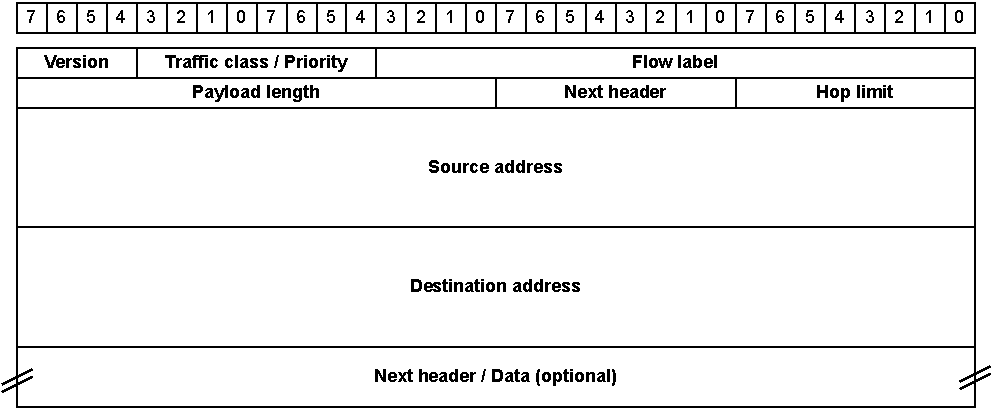
\includegraphics[width=0.75\textwidth]{includes/figures/defi_ipv6_header.pdf}
\end{defi}

\begin{bonus}{IPv6-Erweiterungs-Header}
    Optionale Angaben folgen in \emph{IPv6-Erweiterungs-Headern}:

    \begin{tabularx}{\textwidth}{|X|l|l|X|}
        \hline
        Name                                        & Typ & Größe    & Beschreibung                                                                                                                         \\
        \hline
        \hline
        \emph{Hop-By-Hop Options}                   & 0   & variabel & Enthält Optionen, die von allen IPv6-Geräten, die das Paket durchläuft, beachtet werden müssen. Wird z. B. für Jumbograms benutzt.   \\
        \hline
        \emph{Routing}                              & 43  & variabel & Durch diesen Header kann der Weg des Paketes durch das Netzwerk beeinflusst werden, er wird unter anderem für Mobile IPv6 verwendet. \\
        \hline
        \emph{Fragment}                             & 44  & 64 Bit   & In diesem Header können die Parameter einer Fragmentierung festgelegt werden.                                                        \\
        \hline
        \emph{Authentication Header (AH)}           & 51  & variabel & Enthält Daten, welche die Vertraulichkeit des Paketes sicherstellen können.                                                          \\
        \hline
        \emph{Encapsulating Security Payload (ESP)} & 50  & variabel & Enthält Daten zur Verschlüsselung des Paketes.                                                                                       \\
        \hline
        \emph{Destination Options}                  & 60  & variabel & Enthält Optionen, die nur vom Zielrechner des Paketes beachtet werden müssen.                                                        \\
        \hline
        \emph{Mobility}                             & 135 & variabel & Enthält Daten für Mobile IPv6.                                                                                                       \\
        \hline
        \emph{No Next Header}                       & 59  & leer     & Dieser Typ ist nur ein Platzhalter, um das Ende eines Header-Stapels anzuzeigen.                                                     \\
        \hline
    \end{tabularx}
\end{bonus}